\documentclass{beamer}
%\usepackage[latin1]{inputenc}

% Cyrillic support
\usepackage{mathtext}
\usepackage[T2A]{fontenc}
\DeclareSymbolFont{T2Aletters}{T2A}{cmr}{m}{it}
\usepackage[utf8]{inputenc}

% AMS font faces
\usepackage{amsmath, amsfonts, amssymb}

\usetheme{Warsaw}
\title{Гипероктаэдральные комбинаторные типы}
\author{Сергей Воробьев}
\institute{Санкт-Петербургский Государственный университет}
\date{2012}
\begin{document}

\begin{frame}
\titlepage
\end{frame}


\begin{frame}{Введение}
Обычные species $\widehat{\mathbb B}$
$$
F\colon \mathbb{B} \rightarrow \mathbf{Set}
$$
\begin{figure}
   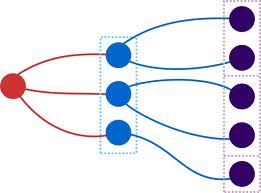
\includegraphics{species.jpg}
\end{figure}

\end{frame}

\end{document}
